% !TEX TS-program = pdflatex
\documentclass[aspectratio=169,11pt]{beamer}
\usetheme{metropolis}
\metroset{sectionpage=none, numbering=none, progressbar=frametitle}

\usepackage[T1]{fontenc}
\usepackage[utf8]{inputenc}
\usepackage{booktabs}
\usepackage{graphicx}
\usepackage{textcomp}

\title{V-KEMS}
\subtitle{The Virtual Forum for Knowledge Exchange in the Mathematical Sciences}
\author{Jess Enright \\ \small co-chair, V-KEMS}
\institute{School of Computing Science, University of Glasgow}
\date{KE Hub Seminar Series \\ 24 September 2026}

\begin{document}

\maketitle

\section{March 2020}

\begin{frame}{March 2020}
  \centering
  \vfill
  \setlength{\tabcolsep}{2pt}
  \renewcommand{\arraystretch}{1.1}
  \begin{tabular}{@{}ccc@{}}
    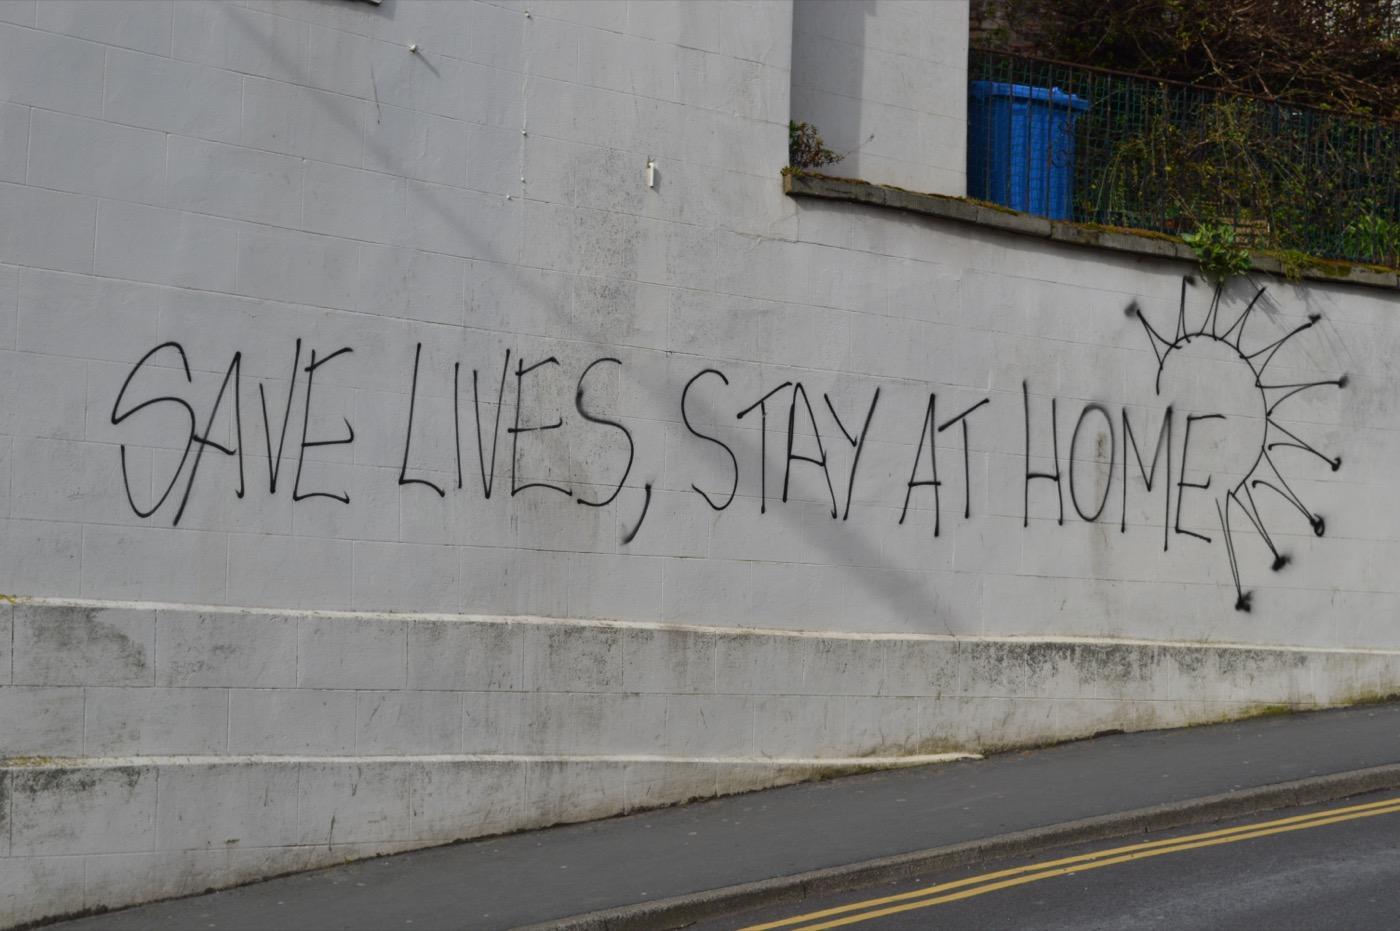
\includegraphics[height=0.40\textheight]{graffiti.jpg} &
    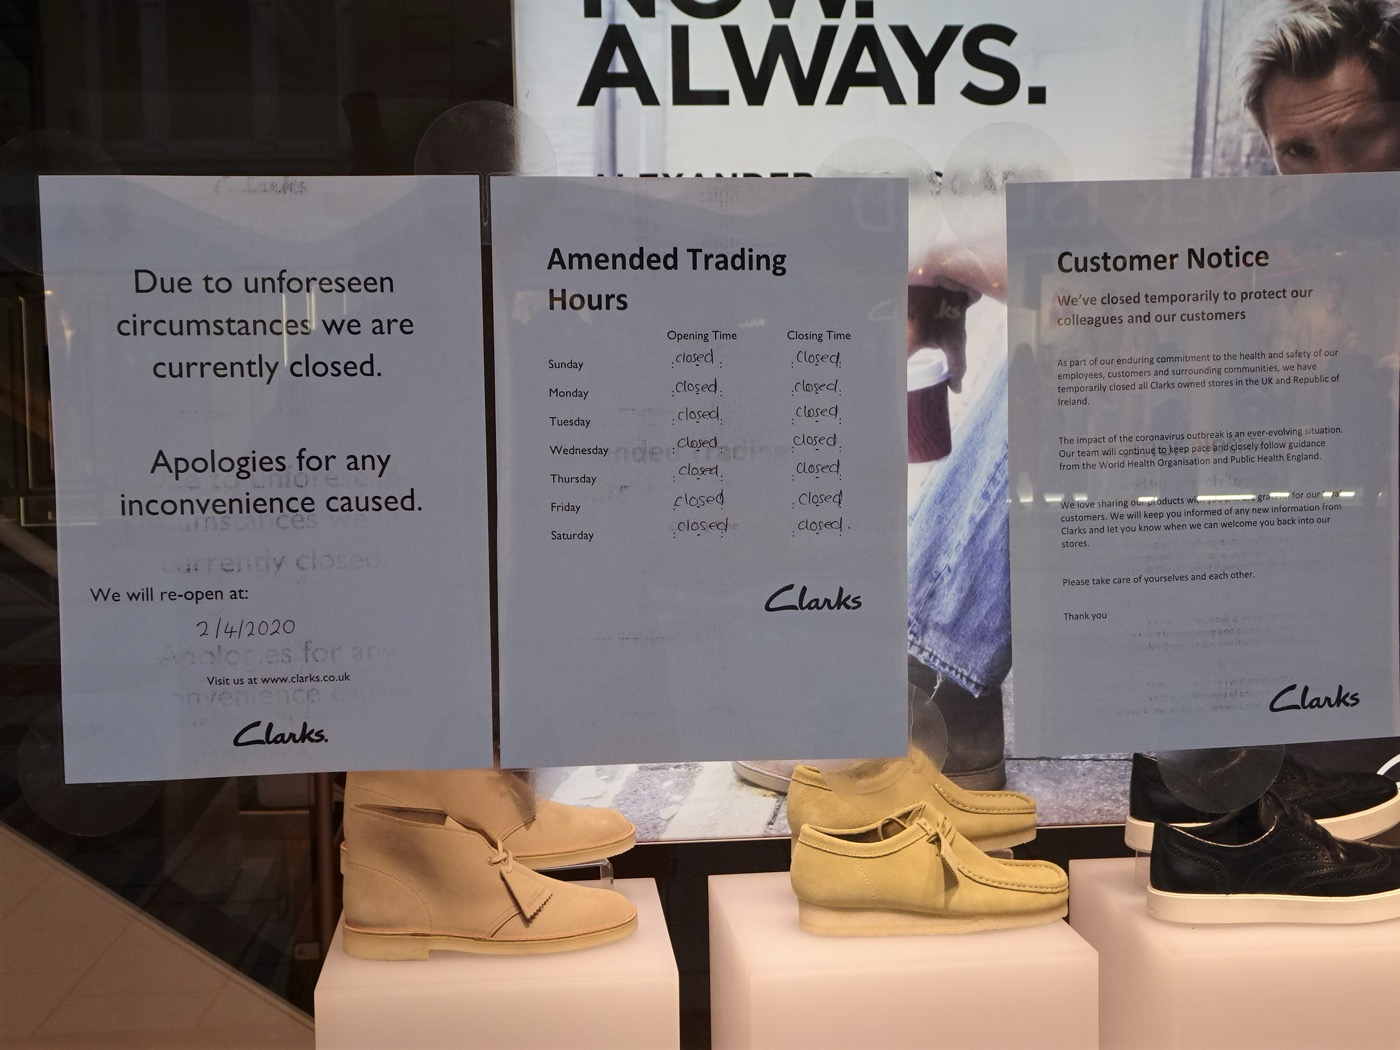
\includegraphics[height=0.40\textheight]{clarkes-closed.jpg} &
    
\includegraphics[height=0.40\textheight]{gov-alert-crop.png} \\[0.3em]
    {\small Whitby, 15 March} &
    {\small Cardiff, 18 March} &
    {\small Every UK phone, 24 March} \\
  \end{tabular}
  \vfill
  {\tiny Via Wikimedia Commons: Zakhx150 (CC BY-SA 4.0) \textbullet\ Sionk (CC BY-SA 4.0)
  \textbullet\ UK Government (public domain)\par}
\end{frame}

\begin{frame}{V-KEMS: set up in March 2020}
  A collaboration between
  \begin{itemize}
    \item Isaac Newton Institute
    \item Newton Gateway to Mathematics
    \item International Centre for Mathematical Sciences
    \item KTN, now Innovate UK Business Connect
  \end{itemize}
  \vfill
  \begin{columns}[T]
    \begin{column}{0.5\textwidth}
      \textbf{First VSG}: 20--23 April\\
      2 industrial problems, 30 people
    \end{column}
    \begin{column}{0.5\textwidth}
      \textbf{Second VSG}: 29--30 April\\
      50 people, and a 50-page report to\\ government two days later
    \end{column}
  \end{columns}
\end{frame}

\begin{frame}{Virtual was both required and beneficial}
  Our June 2020 operations manual noted that being online meant more people could take part:
  \begin{itemize}
    \item people with caring responsibilities
    \item people with unavoidable work commitments
    \item people who could not travel
    \item domain experts who were only needed for part of the time
  \end{itemize}
  \vfill

  \vfill
  Online activities were part of our founding, and remain part of our focus.
\end{frame}

\begin{frame}{Why am I giving this talk?}
\textbf{I want two things from you}

  \begin{columns}[T]
    \begin{column}{0.5\textwidth}
      \textbf{If you are an academic}

      \vspace{1em}
      Come and take part.
    \end{column}
    \begin{column}{0.5\textwidth}
      \textbf{If you are not}

      \vspace{1em}
      Bring us a problem.
    \end{column}
  \end{columns}
  \vfill
  Let me show you why both are worth doing.
\end{frame}

\section{How a study group actually works}

\begin{frame}{How a virtual study group works}
  \begin{itemize}
    \item \textbf{Day 1:} each problem owner presents their problem
      (20 minutes, plus questions)
    \item Participants pick which problem they want to work on
    \item Teams usually split up into smaller groups of 4-5
    \item Short progress updates each morning, and a catch-up at the end of the day
    \item \textbf{Last day:} each team presents what they've done, and
      afterwards writes a report
  \end{itemize}
  \vfill
  There's (ideally) funding available to keep working on problems afterwards.
\end{frame}

\begin{frame}{What it costs you}
  \begin{columns}[T]
    \begin{column}{0.5\textwidth}
      \textbf{Problem owner}

      \vspace{0.8em}
      Some time in advance preparing the problem and any data - we can help with this.  
      
      \vspace{0.8em}
      Twenty minutes of presentation, be reachable during the three days, and attend final presentations.

      \vspace{0.8em}
   %   \alert{Preferably no protected data.  Open problems only.}
    \end{column}
    \begin{column}{0.5\textwidth}
      \textbf{Participant}

      \vspace{0.8em}
      
      Be comfortable with "mutually assured ignorance", and willing to engage.
      
       \vspace{0.8em}
      You do not have to commit the whole week, but more time is better.

      \vspace{0.8em}
      Come for the part where you are useful: this might be most of it!  Some time after the event will also be needed.
    \end{column}
  \end{columns}
\end{frame}

\begin{frame}{When a VSG might be the wrong tool}
  \begin{itemize}
    \item The problem cannot be discussed openly
    \item The data cannot be shared in any form, or does not exist yet
    \item You need a guaranteed answer by a fixed date
    \item It is not really amenable to mathematical formulation 
  \end{itemize}
  \vfill
  We can usually quickly help a problem owner figure out what their best use of a VSG is
  before they commit anything.
\end{frame}

\section{Four study groups}
\begin{frame}{I want to tell you about some of our past activities}
\begin{itemize}
\item Pandemic crisis era: unlocking higher education
\item Pandemic-adjacent: cardiovascular waiting lists
\item Post-crisis: future of the high street
\item More recent: archaeology
\end{itemize}
\end{frame}

\begin{frame}{Unlocking Higher Education Spaces}
  \textbf{June 2020} \quad\textbar\quad Newton Gateway

  \vspace{1em}
  How do you reopen a campus?
  \vfill
  \begin{columns}[T]
    \begin{column}{0.5\textwidth}
      \textbf{Universities got} \\
      a briefing document and a working paper, while they were deciding
      how to reopen
    \end{column}
    \begin{column}{0.5\textwidth}
      \textbf{The mathematicians got} \\
      an interesting new problem - and some of the discussions fed into
      later work on transmission in student populations
    \end{column}
  \end{columns}
\end{frame}

\begin{frame}{...and it led to a paper}
  Discussions at the study group carried on, and turned into this:
  \vfill
  \begin{columns}[c]
    \begin{column}{0.46\textwidth}
      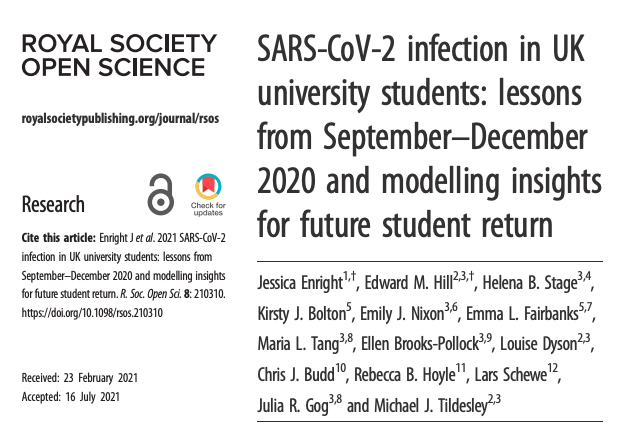
\includegraphics[width=\linewidth,height=0.55\textheight,keepaspectratio]{rsos-student-return.png}
    \end{column}
    \begin{column}{0.52\textwidth}
      \centering
      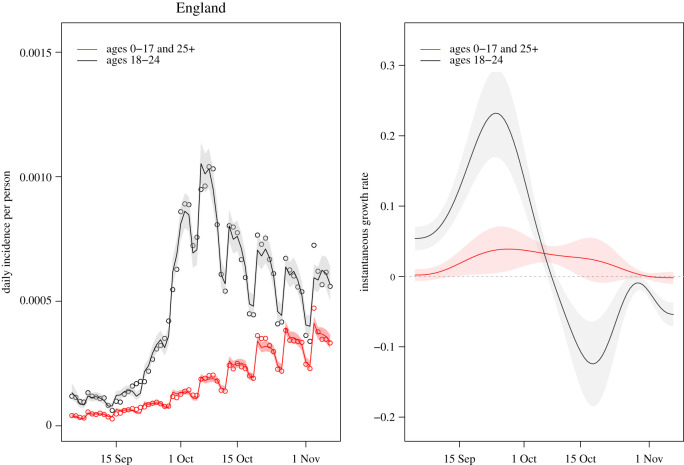
\includegraphics[width=\linewidth,height=0.5\textheight,keepaspectratio]{rsos210310f19.jpg}

      {\tiny Cases in 18--24 year olds (black) and everyone else (red),
      England, autumn 2020\par}
    \end{column}
  \end{columns}
  \vfill
  {\tiny Enright, Hill \emph{et al.} (2021) \emph{R. Soc. Open Sci.} 8:210310,
  CC BY 4.0}
\end{frame}

\begin{frame}{Cardiovascular waiting lists}
  \textbf{February 2021} \quad\textbar\quad NHS, Newton Gateway

  \vspace{1em}
  How has COVID affected cardiovascular waiting lists, and what can be done
  about it?
  \vfill
  \begin{columns}[T]
    \begin{column}{0.5\textwidth}
      \textbf{The NHS got} \\
      models of the referral, diagnosis and treatment pathway, to help plan
      how to bring waiting lists down
    \end{column}
    \begin{column}{0.5\textwidth}
      \textbf{The mathematicians got} \\
      two papers in \emph{BMJ Open} (and I got to be on a podcast!)
    \end{column}
  \end{columns}
\end{frame}

\begin{frame}{What did the models say?}
  One example: waiting lists for aortic stenosis treatment
  \vfill
  \begin{columns}[c]
    \begin{column}{0.36\textwidth}
      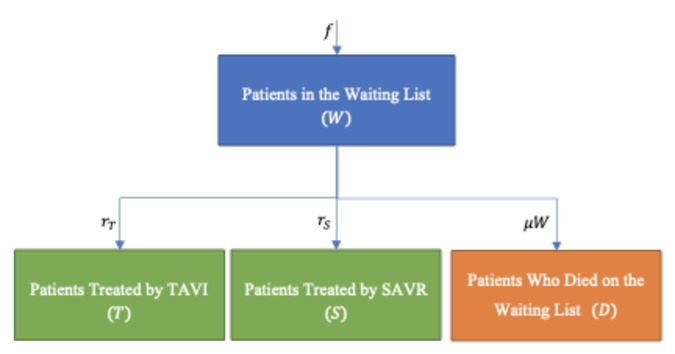
\includegraphics[width=\linewidth]{bmjopen-2021-059309f01.jpg}
    \end{column}
    \begin{column}{0.62\textwidth}
      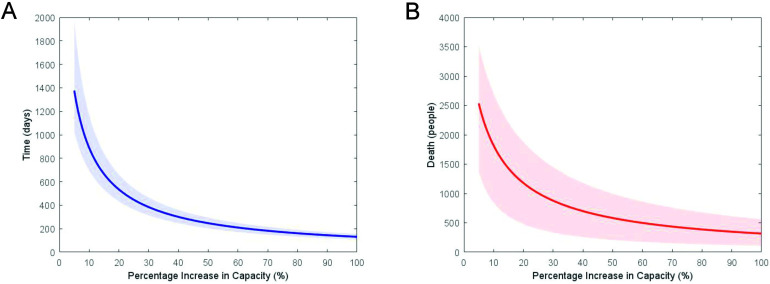
\includegraphics[width=\linewidth]{bmjopen-2021-059309f02.jpg}

      {\scriptsize Time to clear the backlog (left) and deaths on the waiting
      list (right), against the increase in treatment capacity\par}
    \end{column}
  \end{columns}
  \vfill
  Even a modest increase in capacity makes a big difference, both to how long
  the backlog takes to clear and to how many people die waiting.
  \vfill
  {\tiny Stickels, Nadarajah \emph{et al.} (2022) \emph{BMJ Open} 12:e059309,
  CC BY 4.0}
\end{frame}

\begin{frame}{The Future of the High Street}
  \textbf{May 2024} \quad\textbar\quad Innovate UK Business Connect

  \vspace{1em}
  %Not everything we do is about pandemics! Challenges included:
  \begin{columns}[c]
    \begin{column}{0.44\textwidth}
      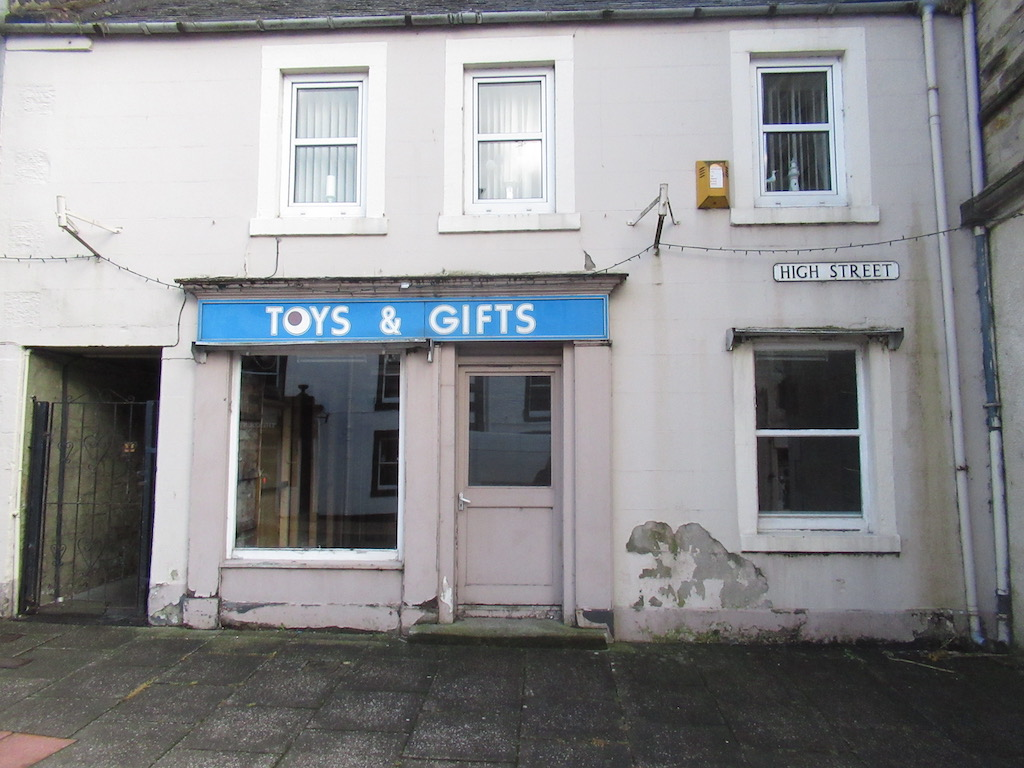
\includegraphics[width=\linewidth]{selkirk-closed-shop.jpg}

      {\tiny High Street, Selkirk, 2022. Richard Webb, CC BY-SA 2.0, via Geograph\par}
    \end{column}
    \begin{column}{0.54\textwidth}
      \begin{itemize}
        \item What does out-of-town shopping do to city centres?
        \item What are the benefits of more people living in Scottish city
          centres? (from the Scottish Cities Alliance)
      \end{itemize}
    \end{column}
  \end{columns}
  \vfill
  Two reports came out of this one.
\end{frame}

\begin{frame}{Where do people in Glasgow shop?}
  \begin{columns}[c]
    \begin{column}{0.55\textwidth}
      \centering
      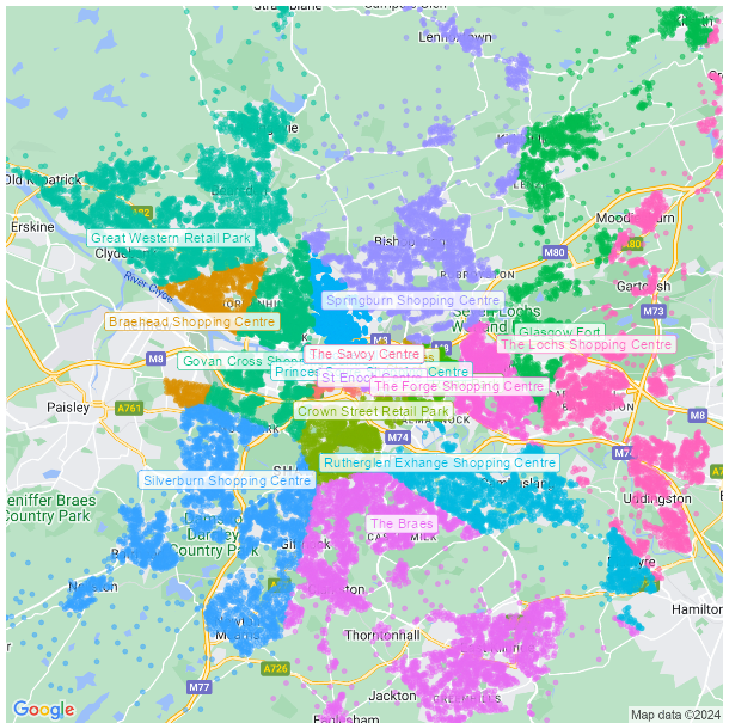
\includegraphics[width=\linewidth,height=0.58\textheight,keepaspectratio]{hs-glasgow-map.png}

      {\tiny Glasgow, split up by nearest shopping area\par}
    \end{column}
    \begin{column}{0.42\textwidth}
      \centering
      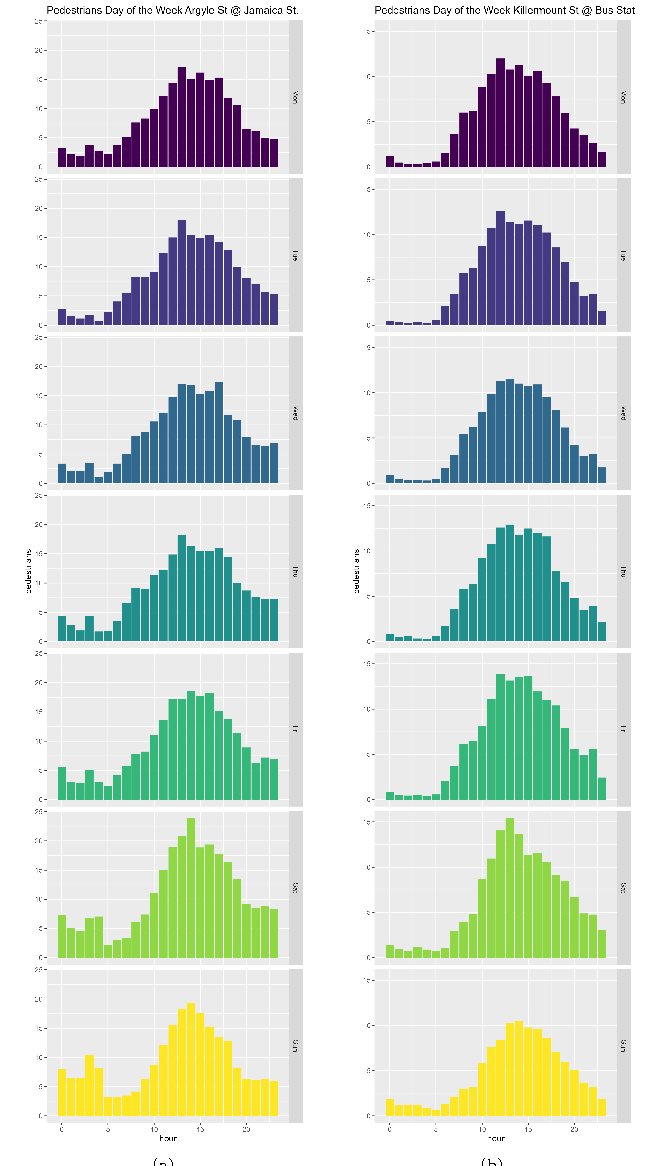
\includegraphics[height=0.58\textheight,keepaspectratio]{hs-glasgow-footfall.png}

      {\tiny Pedestrians by hour, for each day of the week: Argyle St (left) and
      Killermont St (right), from Glasgow's open CCTV counts\par}
    \end{column}
  \end{columns}
  \vfill
  {\tiny From the V-KEMS report on this study group. Map data \copyright\ 2024 Google.\par}
\end{frame}

\begin{frame}{Mathematics in Archaeology and Museum Collections}
  \textbf{September 2025} \quad\textbar\quad Institute for Mathematical
  Innovation, Fitzwilliam Museum

  \vspace{1em}
  \begin{columns}[c]
    \begin{column}{0.44\textwidth}
      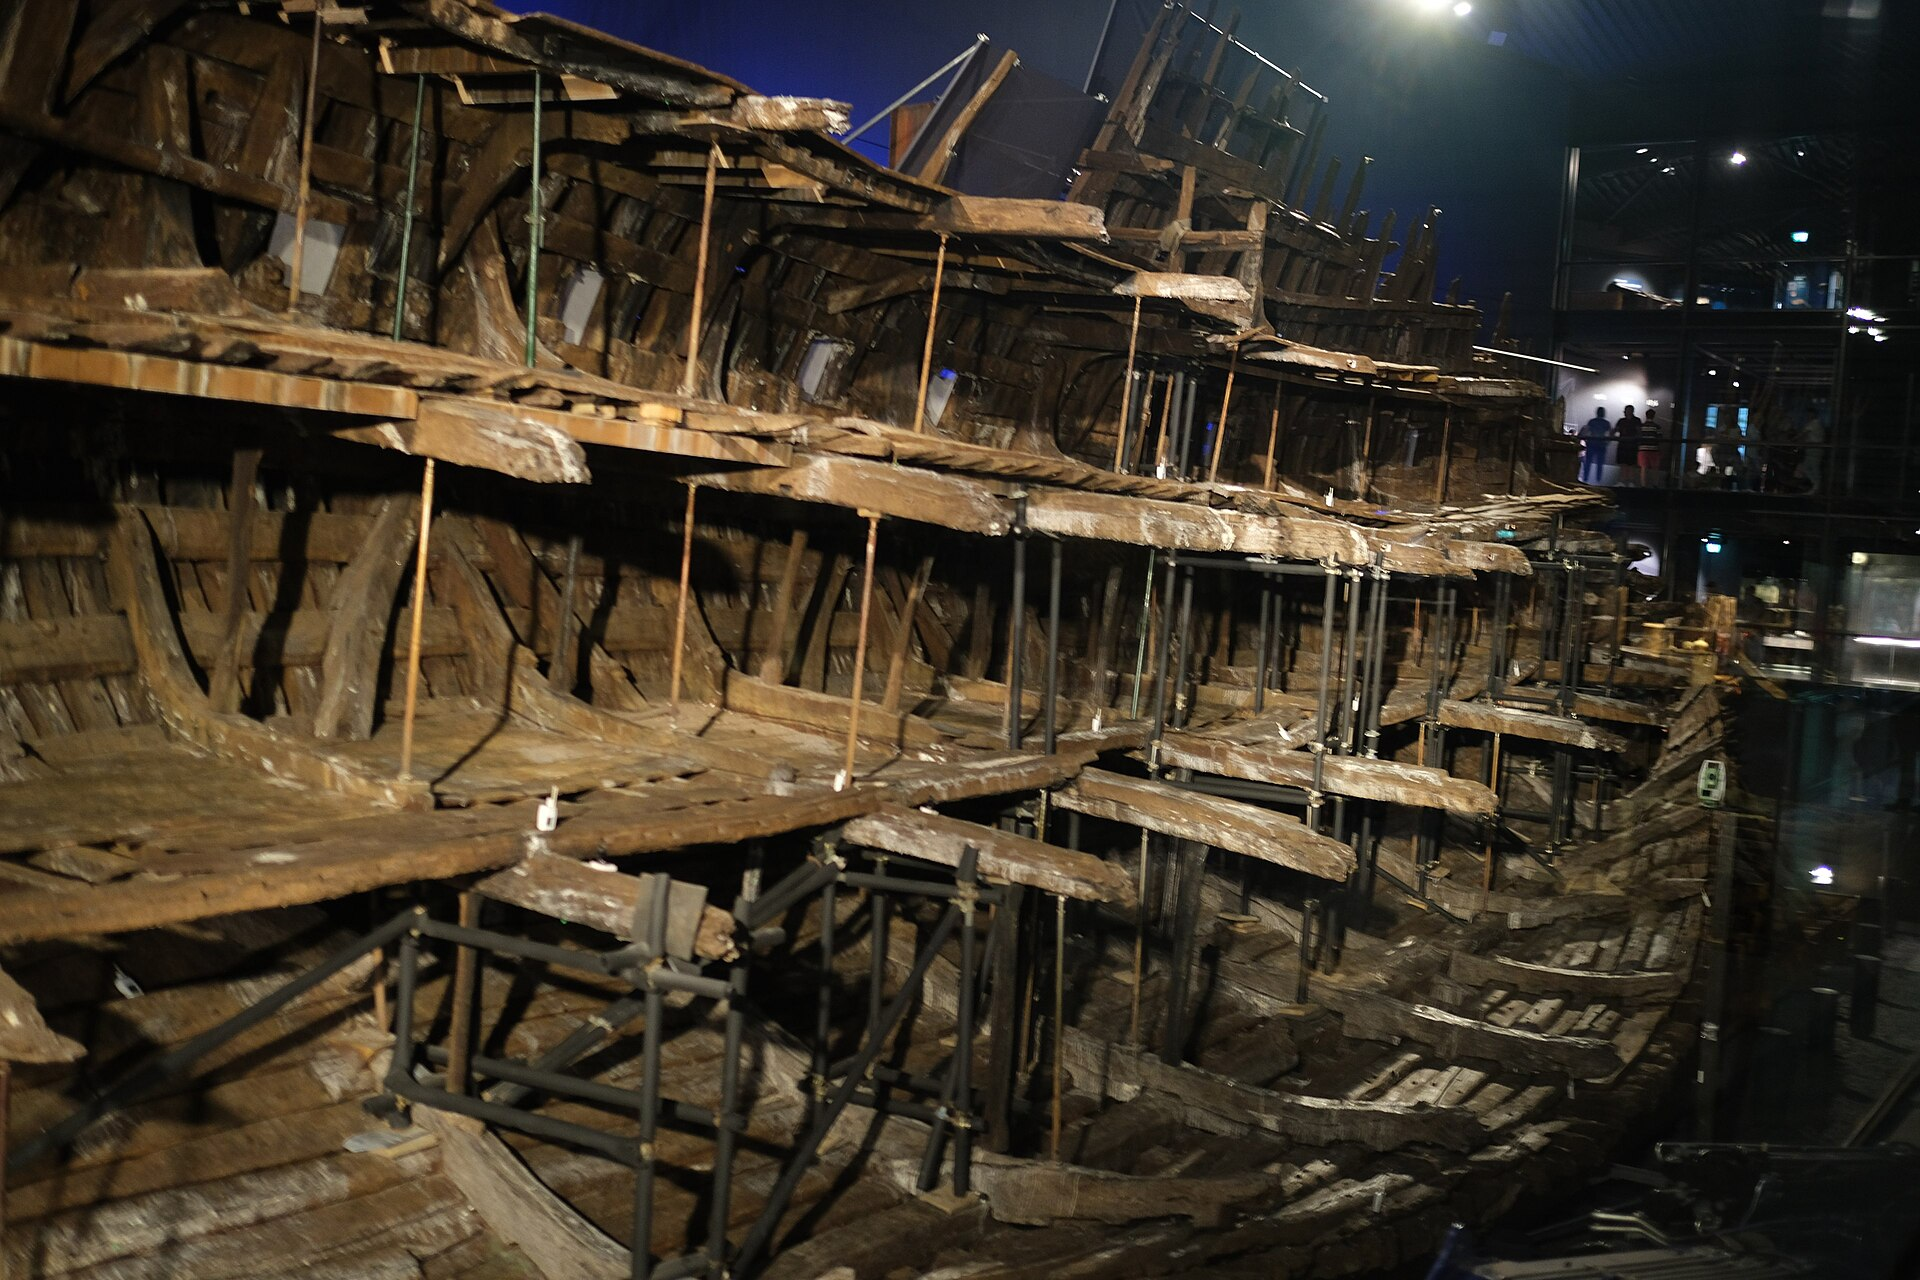
\includegraphics[width=\linewidth]{mary-rose-hull.jpg}

      {\tiny The hull of the Mary Rose. Bob Harvey, CC BY-SA 2.0, via Geograph\par}
    \end{column}
    \begin{column}{0.54\textwidth}
      \begin{itemize}
        \item Energy use at the Mary Rose Museum
        \item Inheritance patterns in Roman Britain, from ancient DNA
        \item Image registration and stitching for cultural heritage
      \end{itemize}
    \end{column}
  \end{columns}
\end{frame}

\begin{frame}[standout]
  Would you have guessed that\\ the Mary Rose Museum\\ had a maths problem?
\end{frame}

\begin{frame}{A Tudor warship and an Egyptian papyrus}
  \begin{columns}[c]
    \begin{column}{0.49\textwidth}
      \centering
      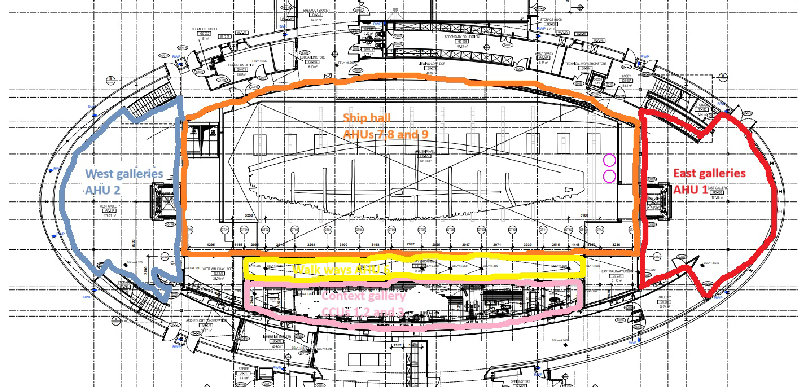
\includegraphics[width=\linewidth]{mr-layout.png}

      {\tiny The Mary Rose has to be kept at 18--20\,\textdegree C and 50--58\%
      humidity. What drives the museum's energy use?\par}
    \end{column}
    \begin{column}{0.49\textwidth}
      \centering
      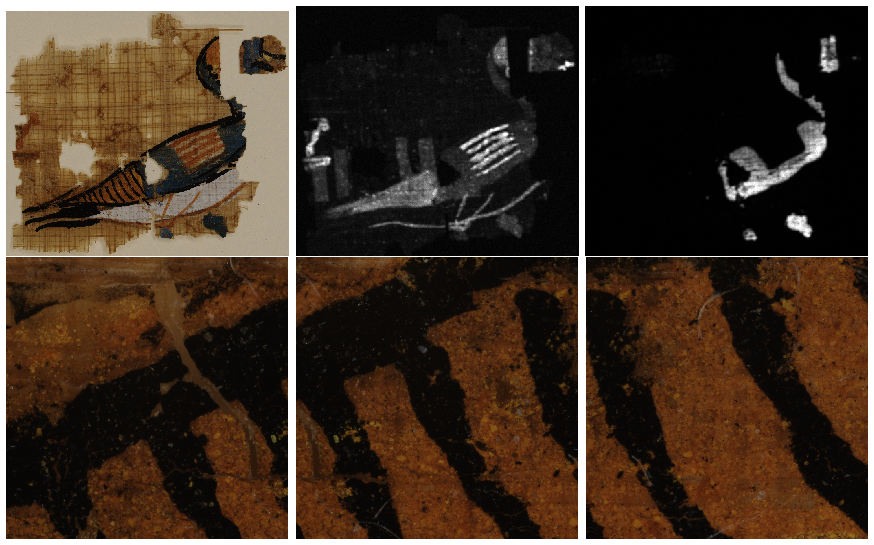
\includegraphics[width=\linewidth]{ir-ramose-modalities.png}

      {\tiny Fragments of the Book of the Dead of Ramose (c.\ 1300 BC) under
      different imaging methods - how do you line the images up?\par}
    \end{column}
  \end{columns}
  \vfill
  {\tiny Figures from the study group reports. Right: \copyright\ Fitzwilliam
  Museum, University of Cambridge.\par}
\end{frame}

\section{Six years on}

\begin{frame}{Where are we now?}
  \begin{itemize}
    \item More than 20 virtual study groups since 2020
    \item On water, food security, justice, higher education funding,
      museums, and lots more
    \item KE Team of the Year at the PraxisAuril awards in 2021
    \item Next up: policing problems, with the NPCC, in December
  \end{itemize}
  \vfill
  We started as a COVID response, but we've kept going!
\end{frame}

\begin{frame}{Coming up: policing problems}
  \textbf{1--3 December 2026} \quad\textbar\quad online, three days

  With the National Police Chiefs' Council and the Policing Academic Centres
  of Excellence, based on the NPCC's \emph{Policing Problem Book}

  \vspace{0.6em}
  Three challenges (details still provisional):
  \begin{itemize}
    \item How does the risk of crime escalate with age, after petty crime in
      youth?
    \item Measuring and reducing systemic bias - e.g. in stop and search
    \item Logistics: drone routing, airspace coordination, where to put assets
  \end{itemize}
  \vfill
  If you'd like to take part, keep an eye on vkemsuk.org!
\end{frame}

\begin{frame}{What might we do in the future?}
  % TODO (Jess): I drafted this from the activities listed on vkemsuk.org -
  % replace with what V-KEMS is actually planning.
  \begin{itemize}
    \item \textbf{Virtual study groups} - still our main activity
    \begin{itemize}
    \item trialling: coupling these with regular online working groups
    \end{itemize}
    \item \textbf{Hybrid study groups} - some people in the room, others online
    \item \textbf{Webinars and scoping meetings} - shorter, to work out whether a
      problem is a good fit
    \item \textbf{Ongoing collaboration with the KE ecosystem} - e.g. KE Hub, Academy
  \end{itemize}
\end{frame}

\begin{frame}{Please get involved!}
  \begin{columns}[T]
    \begin{column}{0.5\textwidth}
      \textbf{Academics}

      \vspace{0.8em}
      Sign up for a study group - and come for as much of it as you can. Early career colleagues especially welcome!
    \end{column}
    \begin{column}{0.5\textwidth}
      \textbf{Everyone else}

      \vspace{0.8em}
      Get in touch with your problems, even if they're not fully formed yet.
    \end{column}
  \end{columns}
  \vfill
  \begin{center}
    \Large \alert{vkemsuk.org}
  \end{center}
\end{frame}

\begin{frame}{Want to join us? We're recruiting!}
  We're looking for an \textbf{early career researcher} to join the V-KEMS
  organising committee, leading on \textbf{communications and marketing}.

  \vspace{0.8em}
  \begin{itemize}
    \item Build your network and get committee leadership experience
    \item Help connect mathematics with real-world problems
    \item Voluntary and unpaid, like all our committee roles
  \end{itemize}
  \vfill
  \textbf{Deadline: 5pm, Wednesday 14 October 2026}

  Details on the Events \& Opportunities page at vkemsuk.org
\end{frame}

\begin{frame}[standout]
  Questions
\end{frame}

\end{document}
